\documentclass[11pt]{article}
\usepackage{amsmath, amssymb, amsthm}
\usepackage[retainorgcmds]{IEEEtrantools}

\usepackage[pdftex]{graphicx}
\usepackage{tikz}
\usetikzlibrary{intersections, calc}

\usepackage{fancyhdr}

%Listings stuff
\usepackage{listings}
\usepackage{lstautogobble}
\usepackage{color}

\definecolor{gray}{rgb}{0.5,0.5,0.5}
\lstset{
basicstyle={\small\ttfamily},
tabsize=3,
numbers=left,
numbersep=5pt,
numberstyle=\tiny\color{gray},
stepnumber=2,
breaklines=true
}

%Format stuff
\pagestyle{fancy}
\headheight 35pt

%Header info
\chead{\Large \textbf{Complex Exponentials}}
\lhead{}
\rhead{}

\begin{document}
\section{Simple Harmonic Motion}
	Trigonometric functions have certain failings when describing SHM, mainly that they can conceal the 3 necessary arguments: amplitude, frequency, and phase. Consider the phase for the functions $\cos \theta$ and $\sin \theta$: the sine function disguises the fact that it is actually SHM shifted by $\pi / 2$.
	\begin{equation}
		\ddot{x} + \omega_0^2 x  = 0
	\end{equation}
	There is an alternative solution to this differential equation, not the cosine function:
	\begin{equation}
		x(t) = e^{i\omega_0 t}
		\label{shmcomplex}
	\end{equation}
	
\section{Complex Analysis}
	Complex numbers in the form $z = x + iy$ can be expressed in \textbf{Cartesian form} as $(x, y)$ and have the following relevant properties:
	\subparagraph{Addition}
		\begin{equation}
			z_1 + z_2 = (x_1 + x_2, y_1 + y_2)
		\end{equation}
		
	\subparagraph{Multiplication}
		\begin{IEEEeqnarray}{rCl}
			z_1 * z_2 & = & (x_1 + iy_1)(x_2 + iy_2)\\
			& = & (x_1x_2 - y_1y_2 + iy_1x_2 + ix_1y_2)\\
			& = & (x_1x_2 - y_1y_2, y_1x_2 + x_1y_2)
		\end{IEEEeqnarray}
		
	\subparagraph{Complex Conjugate}
		\begin{equation}
			z^* = (x + iy)^* = x - iy
		\end{equation}
		\begin{equation}
			zz^* = x^2 + y^2
		\end{equation}
		
	\subparagraph{Division}
		\begin{equation}
			\frac{n}{z} = \frac{nz^*}{zz^*} = \frac{nz^*}{x^2 + y^2}
		\end{equation}
		
	To understand the complex exponential in context of SHM, expand the Taylor series for the expression $e^z$, where for this application we set $z = iy$.
	\begin{IEEEeqnarray}{rCl}
		e^{iy} & = & 1 + iy - \frac{1}{2}y^2 + \frac{1}{3!}iy^3 + \ldots\\
		& = & (1 - \frac{1}{2}y^2 + \frac{1}{4}y^4 + \ldots) + i(y - \frac{1}{3!}y^3 + \frac{1}{5!}y^5 + \ldots)\\
		& = & \cos y + i\sin y\label{eulerproof}
	\end{IEEEeqnarray}
	
	The identity in (\ref{eulerproof}) is called \textbf{Euler's Formula}:
	\begin{equation}
		e^{i\theta} = \cos\theta + i\sin\theta
	\end{equation}
		
\section{Complex Vectors}
	Think of $e^{i\theta}$ as a description of a vector in the complex plane inside a unit circle.
	
	\begin{center}
	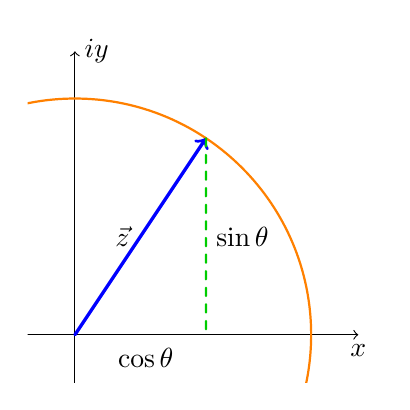
\begin{tikzpicture}
		[scale=3,line cap=round,
		%Styles
		axes/.style=,
		important line/.style={very thick},
		information text/.style={rounded corners,fill=red!10,inner sep=1ex},
		dot/.style={circle,inner sep=1pt,fill,label={#1},name=#1}			
		]
		
		%Colors
		\colorlet{anglecolor}{green!50!black}	%angle arcs/lines
		
		%The graphic
		\clip (-.2, -.2) rectangle (1.3, 1.3);
		
		\draw[<->] (0, -1.2) -- (0, 1.2) node[right] {$iy$};
		\draw[<->] (-1.2, 0) -- (1.2, 0) node[below] {$x$};
		
		\draw[orange,thick] (0, 0) circle (1);		
		
		\coordinate (A) at (1.2, 1.8);
		
		\path [name path=vector] (0,0) -- (A);
		\path [name path=circle] (0, 0) circle (1);
		\path[name path=xaxis](-1, 0) -- (1, 0);
		
		\draw [name intersections={of=vector and circle, by=u},blue,very thick,->]
			(0, 0) -- node[black,left]{$\vec{z}$} (u); 
			
		\path[name path=ycomponent] (u) -- +(0, -3);
		
		\draw[name intersections={of=ycomponent and xaxis, by=v},green!80!black,dashed,thick]
			(u) -- node[right,black] {$ \sin\theta$} (v);
			
		\node[black] at (.3, -.1) {$\cos\theta$};
	\end{tikzpicture}
	\end{center}
	
	Just as in standard trigonometry, the coordinate of $z$ is described as $\cos\theta + \sin\theta$, with the only difference being that the y-component is complex. Then, for any arbitrary $z = x + iy$, we can choose $A = \sqrt{x^2 + y^2}$ and $\theta = \tan^{-1}(y/x)$ so that
	\begin{equation}
		z = x + iy = Ae^{i\theta}
	\end{equation}
	Converting this polar notation to Cartesian notation is done by $x = A\cos\theta,$ and $y = A\sin\theta$.
	
%	\begin{center}
%	\begin{tikzpicture}
%		[scale=3,line cap=round,
%		%Styles
%		axes/.style=,
%		important line/.style={very thick},
%		information text/.style={rounded corners,fill=red!10,inner sep=1ex},
%		dot/.style={circle,inner sep=1pt,fill,label={#1},name=#1}			
%		]
%		
%		%Colors
%		\colorlet{anglecolor}{green!50!black}	%angle arcs/lines
%		
%		%The graphic
%	\end{tikzpicture}
%	\end{center}

%	\begin{figure}[htb]
%		\centering
%		\includegraphics[width=0.8\textwidth]{filename.eps}
%		\caption{Caption.}
%		\label{fig:figure}
%	\end{figure}

%		\def\enotesize{\normalsize}
%		\theendnotes
\end{document}